\documentclass[pdftex,10pt]{beamer}

\useoutertheme{infolines}

\usepackage[ngerman]{babel}
\usepackage[utf8]{inputenc}
\usepackage{times}
\usepackage[T1]{fontenc}
\usepackage{graphicx}
\usepackage[right]{eurosym}
\usepackage{longtable}
\usepackage{bibgerm}
\usepackage{caption}

\usepackage{subcaption}
\usepackage[pdf]{pstricks}
\usepackage{tikz}
\usepackage{neuralnetwork}

\usetikzlibrary{positioning}
\usetikzlibrary{calc}
\usetikzlibrary{fit}
\usetikzlibrary{shapes.geometric}
\usetikzlibrary{shapes.arrows}
\usetikzlibrary{decorations}
\usetikzlibrary{decorations.pathmorphing}
\usetikzlibrary{decorations.text}
\usetikzlibrary{backgrounds}
\usetikzlibrary{intersections}
\usetikzlibrary{plotmarks}
\usetikzlibrary{arrows.meta}

\renewcommand{\footnotesize}{\fontsize{3pt}{4pt}\selectfont}


\graphicspath{{Bilder/}}

\usepackage{pgfplots}
\pgfplotsset{compat=1.10}

\usepackage[european]{circuitikz}
\ctikzset {bipoles/length=1cm}

\setlength{\arrayrulewidth}{0.75pt}

\title[Autonomes Bilderkennungsystem mit neuronalen Netze] {Entwicklung eines autonomen Systems zur Bilderkennung mithilfe Neuronaler Netze auf dedizierter Hardware}

\subtitle{\vspace{0.5cm}Kolloquium - Bachelorarbeit}

\author[Manuel Barky]{Manuel Barkey}

  
\date[Reutlingen, 29.01.2020] 
{Reutlingen, 29.01.2020}

\subject{Mechatronik}


\pgfdeclareimage[height=0.49cm]{logotitel}{./Bilder/Silhouette_HSRT_045K.jpg}
\pgfdeclareimage[height=0.235cm]{logofolie}{./Bilder/hsrt_silhouette_folie.png}
\logo{\pgfuseimage{logotitel}}


% Falls Aufzählungen immer schrittweise gezeigt werden sollen, kann
% folgendes Kommando benutzt werden:

%\beamerdefaultoverlayspecification{<+->}

\begin{document}

\begin{frame}
  \titlepage
\end{frame}

\logo{\pgfuseimage{logofolie}}

%Einleitung soll direkt nach der Titelfolie erfolgen, ohne zusätzliche
%Inhalts- und Inhaltsverlaufsfolien
%
%
%Nach der Einleitung wird vor jedem Abschnitt das Inhaltverzeichnis eingeblendet

\section*{Motivation}\label{sec:motivation}


\begin{frame}{Motivation}

    \begin{columns}[T]
        \column{0.5\columnwidth}
        Spalte 1
        \begin{itemize}
            \item autonomes überwachungssystem, (wild) tiere, tag/nacht geeignet
            \item rasperry pi + infrarotfähiges camera modul
            \item nur mittteilen bei relevanten erkennungen -> NN
            \item on the edge -> spezielle hardware: NCS2
        \end{itemize}
        \column{0.5\columnwidth}
        Spalte 2\\
        irgendwelche bilder
        
    \end{columns}
\end{frame}


\section*{Gliederung}\label{sec:toc}

\AtBeginSection[]
{
  \begin{frame}<beamer>{Gliederung}
    \tableofcontents[currentsection,hideothersubsections]
  \end{frame}
} 

\begin{frame}{Gliederung}
  \tableofcontents[hideallsubsections]
\end{frame}
%
\section[\thesection \  Neuronale Netze]{Neuronale Netze}\label{sec:nn}

% Frame 1
\begin{frame}{Machine Learning}
        Erkennung von Zusammenhängen in großen Datenmengen,\\ohne explizite programmierung darauf.
        \begin{itemize}
            \item Supervised Learning
        \end{itemize}

        \begin{figure}[h]
            \centering
            \def\svgwidth{0.8\columnwidth}
            
\tikzset{
    decision/.style={
        diamond,
        draw,
        text width=4em,
        text badly centered,
        inner sep=-1pt,
        node distance=8em
    },
    block/.style={
        rectangle,
        draw,
        text width=6em,
        %minimum widhth=6em,
        minimum height=5em,
        text centered,
        node distance=20em
    },
    arrow/.style={
        draw,
        >=latex,
        ->
    },
    textfeld/.style={
        %draw,
        text centered,
        node distance=1.5em
    }
}


\begin{tikzpicture}

    
    \node (system) [block] {Klassisches\\Programm};
    \node (system2) [block, right of=system] {Machine Learning\\Programm};

    \node [textfeld, left=of system.162] (inputs) {Daten};
    \node [textfeld, left=of system.198] (regeln) {Regeln};
    \node [textfeld, right=of system] (output) {Ausgaben};

    \node [textfeld, left=of system2.162] (inputs2) {Daten};
    \node [textfeld, left=of system2.198] (output2) {Ausgaben};
    \node [textfeld, right=of system2] (regeln2) {Regeln};
    
    \draw[arrow] (inputs) -- (system.162);
    \draw[arrow] (regeln) -- (system.198);
    \draw[arrow] (system) -- (output);
    
    \draw[arrow] (inputs2) -- (system2.162);
    \draw[arrow] (output2) -- (system2.198);
    \draw[arrow] (system2) -- (regeln2);
    

\end{tikzpicture}

        \end{figure}

        \visible<2->{
        \begin{columns}[T]
        \column{0.3\columnwidth}
        \begin{block}{Neuronale Netze}

        \vspace{0.5cm}
            Für komplexere Input Daten, z.B. Bilder

    \end{block}

    \column{0.65\columnwidth}

    \begin{figure}[h]
        \centering
        \def\svgwidth{\columnwidth}
        \begin{neuralnetwork}[height=1]
    \newcommand{\nodetextclear}[2]{}
    \newcommand{\nodetexth}[2]{$h_#2$}
    \newcommand{\nodetextx}[2]{$x_#2$}
    \newcommand{\nodetexty}[2]{$y_#2$}
    \inputlayer[count=3, bias=false, title=Input\\layer, text=\nodetextx]
    \hiddenlayer[count=4, bias=false, title=Hidden\\layer, text=\nodetexth] \linklayers
    \outputlayer[count=2, title=Output\\layer, text=\nodetexty] \linklayers
\end{neuralnetwork}
    \end{figure}
    \end{columns}
        }
\end{frame}

% Frame 2
\begin{frame}{Training \& Inferenz}
    \begin{columns}[T]
        \column{0.6\columnwidth}
        Training
        \begin{figure}
            \centering
            \def\svgwidth{0.8\columnwidth}
            
\tikzstyle{process} = [rectangle, fill=blue!20, minimum width=2.5cm, minimum height=1cm, text centered, draw=black]
\tikzstyle{arrow} = [thick,->,>=stealth]

\begin{tikzpicture}[node distance=1.6cm]

  \begin{scope}[node distance=2.5cm]
    \node (nn)      [process]                   {Neuronales Netz};
    \node (pred)      [process, below of=nn]      {Vorhersage};
    \node (loss)      [process, below of=pred]      {Fehlerfunktion};
    
  \end{scope}
  
  \begin{scope}[node distance=4cm]
    \node (opt) [process, left of=pred]      {Optimierer};
    \node (weights)  [process, left of=nn] {Gewichte};
    \node (labels)   [process, right of=pred]  {Labels};
  \end{scope}

  \node (input) at (0,1.5) {Input};

  \draw[arrow] (input) -- (nn);

  \draw[arrow] (nn) -- (pred);
  \draw[arrow] (pred) -- (loss);

  \draw[arrow] (labels) |- (loss);
  \draw[arrow] (loss) -| (opt);

  \draw[arrow] (opt) -- (weights);
  \draw[arrow] (weights) -- (nn);
  
    
\end{tikzpicture}

        \end{figure}
        \begin{itemize}
            \item variable Parameter: \textit{Weights}
            \item bekannte Input Daten: \textit{Labels}
            \item mehrfaches durchlaufen: \textit{Epochen}
        \end{itemize}
        \column{0.4\columnwidth}
        \visible<2->{
        Inferenz
        \begin{figure}
            \centering
            \def\svgwidth{0.4\columnwidth}
            \input{Bilder/infer_workflow.pdf_tex}
        \end{figure}
        \begin{itemize}
            \item fixe Parameter
            \item unbekannte Input Daten
            \item einmaliges durchlaufen
        \end{itemize}
        }
    \end{columns}
\end{frame}



\section[\thesection \  Hardware]{Hardware}\label{sec:hardware}

% Frame 4
\begin{frame}{Intel Neural Compute Stick 2}
    \begin{columns}[T]
        \column{0.6\textwidth}
        Beschleuniger für die Inferenz von Deep Learning Algorithmen
        \vspace{0.3cm}
        \begin{itemize}
            \item geeignet für \textbf{Edge Anwendungen} wie:
            \begin{itemize}
                \item Überwachungskameras, Drohnen, \dots
            \end{itemize}
            \end{itemize}
            \begin{itemize}
                
            
            \item Prozessor: \textbf{Intel Movidius Myriad X VPU}
            \begin{itemize}
                \item effizient bei NN-spezifischen Rechenopereationen
            \end{itemize}
            
        \end{itemize}
        \column{0.4\textwidth}
        \vspace{1cm}
        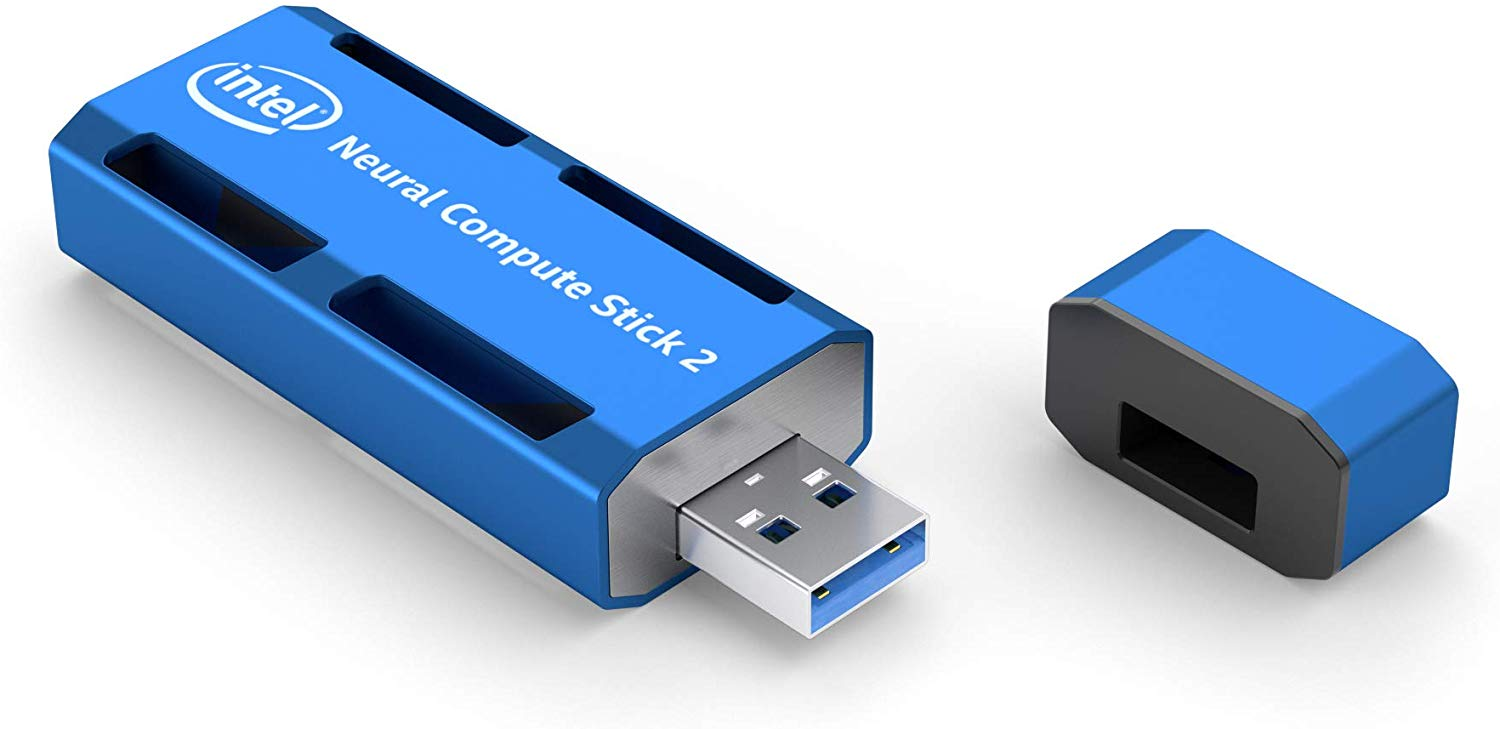
\includegraphics[width=0.8\textwidth]{Bilder/ncs2.jpg}
    \end{columns}
    \vspace{0.3cm}

    \visible<2->{

    \begin{columns}[T]
        \column{0.4\textwidth}

        \begin{block}{OpenVINO Toolkit}
    
            Inferenz auf Intel-Hardware
            \begin{itemize}
                \item Eigenes Dateiformat für Deep Learning Model
                \item Unterstütze Frameworks:
                \begin{itemize}
                    \item  Tensorflow, Caffe
                \end{itemize}
            \end{itemize}
        \end{block}
            \column{0.6\textwidth}
            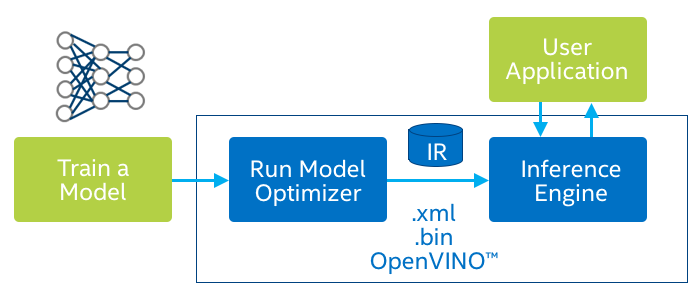
\includegraphics[width=\textwidth]{Bilder/open_vino_workflow_steps.png}
        \end{columns}

    }
        
\end{frame}
\section[\thesection \  Training des Modells]{Training des Modells}\label{sec:training}
%
%--------------------------------------------------------------------
%

\subsection[\thesection .\thesubsection \ 
Deep Learining Computer Vision]{Deep Leaerining Computer Vision}\label{subsec:dl_cv}


% Frame 5
\begin{frame}{Convolutional Neural Networks}

    \begin{figure}
        \centering
        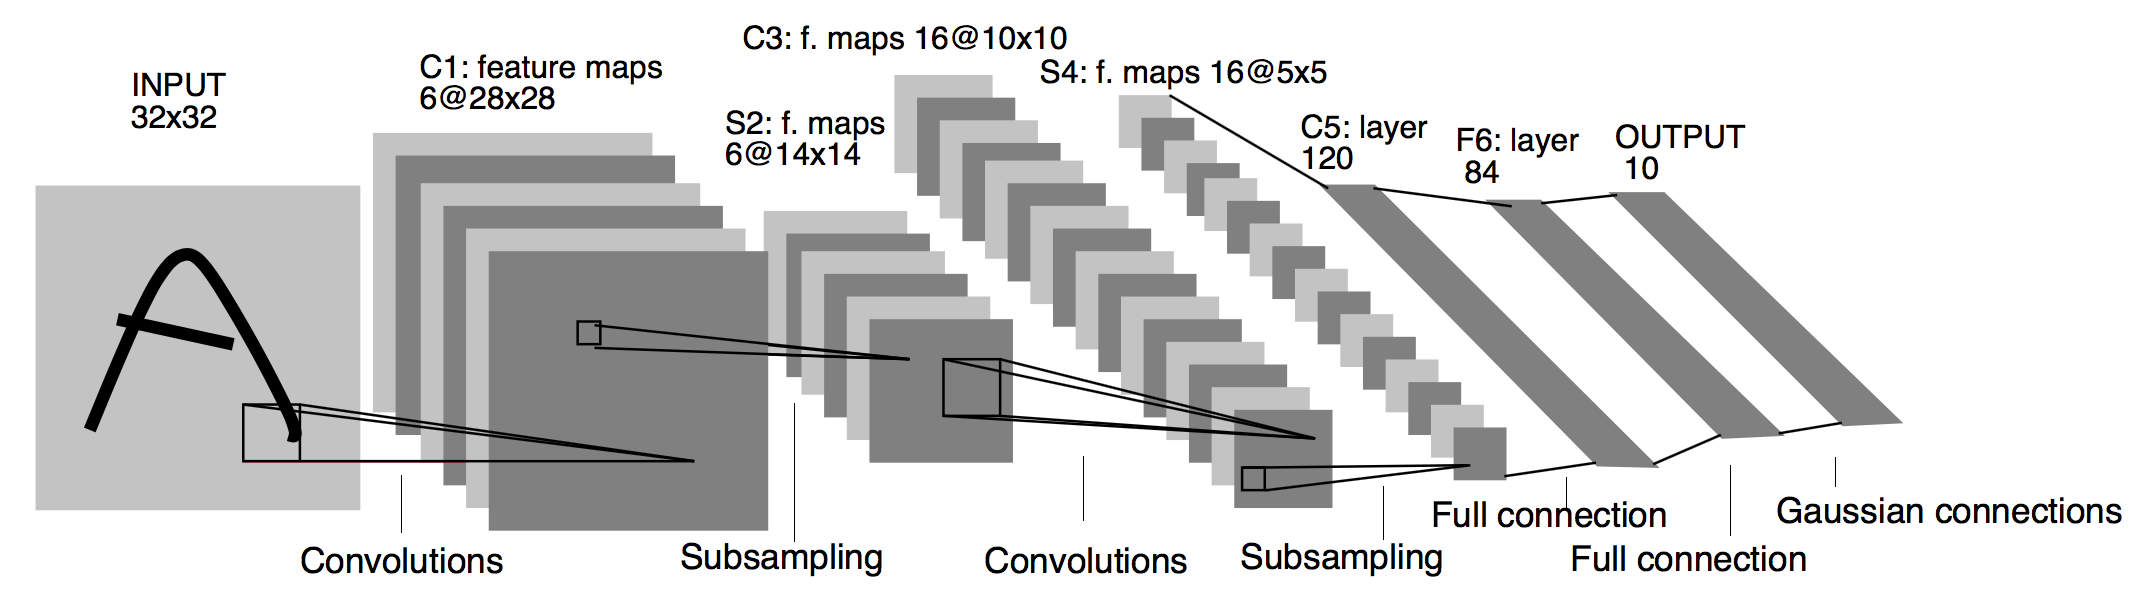
\includegraphics[width=0.7\textwidth]{Bilder/lenet.png}
    \end{figure}

    \begin{columns}[T]
        \column{0.1\columnwidth}
        \column{0.5\columnwidth}
        \begin{itemize}
            \item Convolutional Layers
            \begin{itemize}
                \item extrahieren von Features
                \item Räumliche Invarianz durch Faltung
                \item weniger Parameter durch kernel
            \end{itemize}
        \end{itemize}
        \column{0.5\columnwidth}
        \visible<2->{
        \begin{itemize}
            \item Fully Connected Layers
            \begin{itemize}
                \item Classification
            \end{itemize}
        \end{itemize}}
    \end{columns}
    \vspace{0.5cm}
    \visible<3->{
    \begin{itemize}
        \item Implementierung mithilfe Frameworks wie z.B. Tensorflow
    \end{itemize}}
        


    % \begin{block}{Arten der Erkennung}
    %     classification vs obj erk vs segmentation
    %     \\
    %     graphik
    % \end{block}
\end{frame}


% Frame 6
\begin{frame}{Objekterkennung}

    \begin{columns}[T]
        \column{0.5\columnwidth}

        \begin{itemize}
            \item zusätzliche Lokalisierung der erkannten Objekte im Bild
        \end{itemize}
        \begin{itemize}
            \item verschiedene Architekturen: 
            \begin{itemize}
                \item Regionbased CNNs (zweistufig)
                \item Single Shot Detectoren
            \end{itemize}
            verwenden beide CNNs als \textit{Backbone Networks}
        \end{itemize}

        \column{0.5\columnwidth}

        \begin{figure}
            \centering
            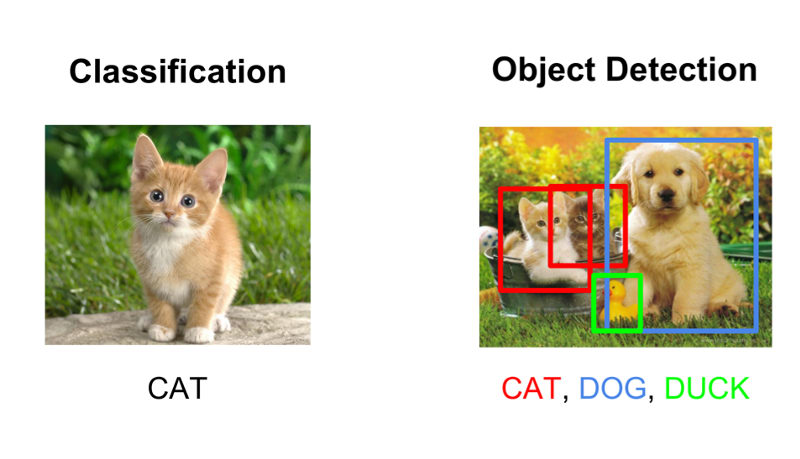
\includegraphics[width=0.9\textwidth]{Bilder/classification_detection.jpeg}
        \end{figure}
        
    \end{columns}

    \vspace{0.5cm}
        \visible<2->{
        \begin{columns}[T]
            \column{0.5\columnwidth}

            \begin{block}{Tensorflow Object Detection Api}

            \begin{itemize}
                \item Trainiert auf
                \begin{itemize}
                    \item SSD und Faster RCNN
                    \item Mobilenet, InceptionV2, Resnet50
                \end{itemize}
            \end{itemize}
        \end{block}

        \column{0.5\columnwidth}
            \begin{figure}
                \centering
                
\includegraphics[width=0.75\textwidth]{Bilder/tf_icon.png}
            \end{figure}
        \end{columns}
        }
        % rechts daneen noch grundstruktur von obj det: cnn -> 1. class, 2. regr (boxen)

\end{frame}



\subsection[\thesection .\thesubsection \ 
Sammeln und aufbereiten der Daten]{Sammeln und aufbereiten der Daten}\label{subsec:collect_data}
% Frame 7
\begin{frame}{Datensatz}
    Objekterkennung: Trainingsdaten mit Bounding Boxkoordinaten gelabelt
    \begin{block}{OpenImages}
        Frei zugängliches Datenset mit 9M Bildern
        \begin{itemize}
            \item 'Brown Bear', 'Deer' 'Fox', und weitere
        \end{itemize}
    \end{block}

    \begin{block}{Validierungs Split}
        Afteilung der Daten in:
        \begin{figure}[h]
            \centering
            \def\svgwidth{0.8\columnwidth}
            \input{Bilder/train_test_split.pdf_tex}
        \end{figure}
        Test- und Validierungs-Set dienen der Kontrolle\\
        \begin{itemize}
            \item Overfitting
        \end{itemize}
    \end{block}
\end{frame}

% Frame 8
\begin{frame}{Aufbereiten der Daten}
    \begin{block}{Augmentierung}
        \begin{itemize}
            \item Geometrisch: Verschieben, Spiegeln, Rotieren, Zoom
            \item oder: Farbwerte, Helligkeit, kontrast, Noise
        \end{itemize}
        Bild von verschiedenen Augmentierungen
    \end{block}
    \begin{block}{Graustufen}
        hier bild (von verschiedenen graustufen und helligkeiten)
    \end{block}
\end{frame}


\subsection[\thesection .\thesubsection \ 
Training]{Training}\label{subsec:train}
% Frame 9
\begin{frame}{Trainingsworkflow}
    Mit den aufbereiteten Daten und dem ausgewählten Model trainieren
    \\
    hier blockdiagramm mit [daten aufberreitung]->[model auswahl]->[trainin]->[evaluiern]->rückführung zu:
    \begin{itemize}
        \item trining: hyperparameter anpassen
        \item model: neues model auswählen
        \item date aufbereiten: andere dasten/augemntierung verwenden
    \end{itemize}
    solange bis passt
    \\
    verwendet:
    \begin{itemize}
        \item Daten: OI, mit/ohne Aug, graustufen
        \item Modelle: ssd, faster rsnn mit Backbone: Mobilenet, inception, restnet
        \item hyperparametrt \dots
    \end{itemize}
\end{frame}


\subsection[\thesection .\thesubsection \ 
Evaluierung]{Evaluierung}\label{subsec:eval}

% Frame 10
\begin{frame}{Metriken}
    Für Objekt Detection müssen 2 Faktoren berücksichtigt werden:
    \begin{itemize}
        \item existiert ein Objekt im Bild: Classificatinon
        \item wo befindet sich das obj: regression (der bbox koordinaten)
    \end{itemize}
    \begin{block}{mAP (für genauigkeit)}
        \begin{itemize}
            \item IoU > 0.5 -> True pos, else: False pos; => prec = TPs / alle Pos
            \item Recall = TPs / TPs + FN (FN falsche klasse getippt)
            \item AP = summe aller P(R) für R 0..1
            \item mAP für alle mittelwert für alle klassen
        \end{itemize}        
    \end{block}
    \begin{block}{Loss (für die Fehler rate)}
        \begin{itemize}
            \item Binärer Log Loss (CrossEntropy) für Box Classification
            \item Regressor für Box Koordinaten
        \end{itemize}
    \end{block}
\end{frame}

% frame 10
\begin{frame}{Metriken}
    Für Objekt Detection müssen 2 Faktoren berücksichtigt werden:
    \begin{itemize}
        \item existiert ein Objekt im Bild: Classificatinon
        \item wo befindet sich das obj: regression (der bbox koordinaten)
    \end{itemize}
    \begin{block}{Für die Genauigkeit}
        IoU berechnung plus graphig, ab best thresshold wird als tp gewertet, sont tn\\
        daraus ergibt sich:\\
        Precision=tp/(tp+fp)\\
        unf recall=tp/tp+fn\\
        (hier nur nicht auf bezeichnungen tp tn \dots eingehen sondern bedeutung für modell erklären)
        \\
        da mit steigendem Precision recall abnimmt, kann die fläche der Precision über recall kurve als AP (average pr) dienen 

    \end{block}
    \begin{block}{Für die Fehlerrate}
        \begin{itemize}
            \item Klassifikation: Binärer Log Loss (CrossEntropy)
            \item Regressor für Lokalisierung
        \end{itemize}
    \end{block}
\end{frame}


% Frame 11
\begin{frame}{Auswirkung von Augmentierung}

    \begin{columns}[T]
        \column{0.05\textwidth}
        \vspace{1.5cm}
        Loss\\
        \vspace{3cm}
        \visible<2->{
        mAP\\
        }

        \column{0.45\textwidth}
        \centering
        ohne Augmentierung
        \begin{figure}
            \centering
            \def\svgwidth{0.75\columnwidth}
            %\fontsize{3pt}{4pt}\selectfont
            \footnotesize
            \input{Bilder/loss_ohne_aug.pdf_tex}
            %\caption{\scriptsize ohne Augmentierung}
        \end{figure}

        \visible<2->{
        \begin{figure}
            \centering
            \def\svgwidth{0.75\columnwidth}
            \footnotesize
            \input{Bilder/mAP_ohne_aug.pdf_tex}
            %\caption{ohne Augmentierung}
        \end{figure}
        }

        \column{0.45\textwidth}
        \centering
        mit Augmentierung

        \begin{figure}
            \centering
            \def\svgwidth{0.75\columnwidth}
            \footnotesize
            \input{Bilder/loss_aug.pdf_tex}
            %\caption{ohne Augmentierung}
        \end{figure}
        \visible<2->{
        \begin{figure}
            \centering
            \def\svgwidth{0.75\columnwidth}
            \footnotesize
            \input{Bilder/mAP_aug.pdf_tex}
            %\caption{ohne Augmentierung}
        \end{figure}
        }

    \end{columns}
    \begin{itemize}
        \fontsize{7pt}{8pt}\selectfont
        \item Training: 200.000 Steps, Faster RCNN + InceptionV2, auf 9 Klassen
    \end{itemize}
\end{frame}

%##########################  CHAPER 6: APPLICATION  #######################

\chapter{Entwicklung der Anwendung}\label{kap:application}


Dieses Kapitel beschreibt die Entwicklung der Anwendung,
welche als autonomes System dass auf einem Raspberry Pi 4 läuft.

Dazu gehören die Einrichtung einer infrarotfähigen 
Kamera, die Implementierung der Inferenz mit OpeVino
und die Verbindung zu einem Pc zur übertragung
der Daten mit geeignetem Protokolls.



%-------------------------  SECTION 1: AUFBAU  ------------------------
\section{Aufbau/Hardware}\label{sec:aufbau}


Der Aufbau besteht aus einem Raspberry Pi, auf welche 
der Anwendungscode läufr, dem NCS2 für die Inferenz, 
welcher per USB mit dem Raspberry verbunden wird.

Desweiteren wurde ein Raspberry Pi Kamera Modul mit 
5MP OV5647 Sensor der Marke Longrunner verwendet.

Dieses ermöglicht durch zu und abschalten eines Infrarot 
Filters vor die Linse zwischen Tag und Nachtsicht zu wechseln.

Das Schalten wird dabei über einen Helligkeitssensor automatisch 
geregelt. Im Infrarotmodus bfindet sich der Infrarot Filter nicht 
vor der linse, wodurch auch die etwas längeren (850nm)
Elektromagnetischen Wellen als die des Sichtbaren Lichts aufgenommen 
werden können.

Durch zwei Infrarot LEDs des gleichen Spektrums, können so 
auch in der Dunkelheit Bilder aufgenommen werden, ohne 
Sichtbare beläuchtung, was Tiere verscheuchen würde.


Das kamera Modul wird über die CSI (Camera Serial Interface) 
Schnittstelle mit dem Raspberry Pi verbunden.


%https://www.amazon.de/gp/product/B07R4JH2ZV/ref=ppx_yo_dt_b_asin_title_o01_s00?ie=UTF8&psc=1


\begin{minipage}{0.55\textwidth}
    \centering
    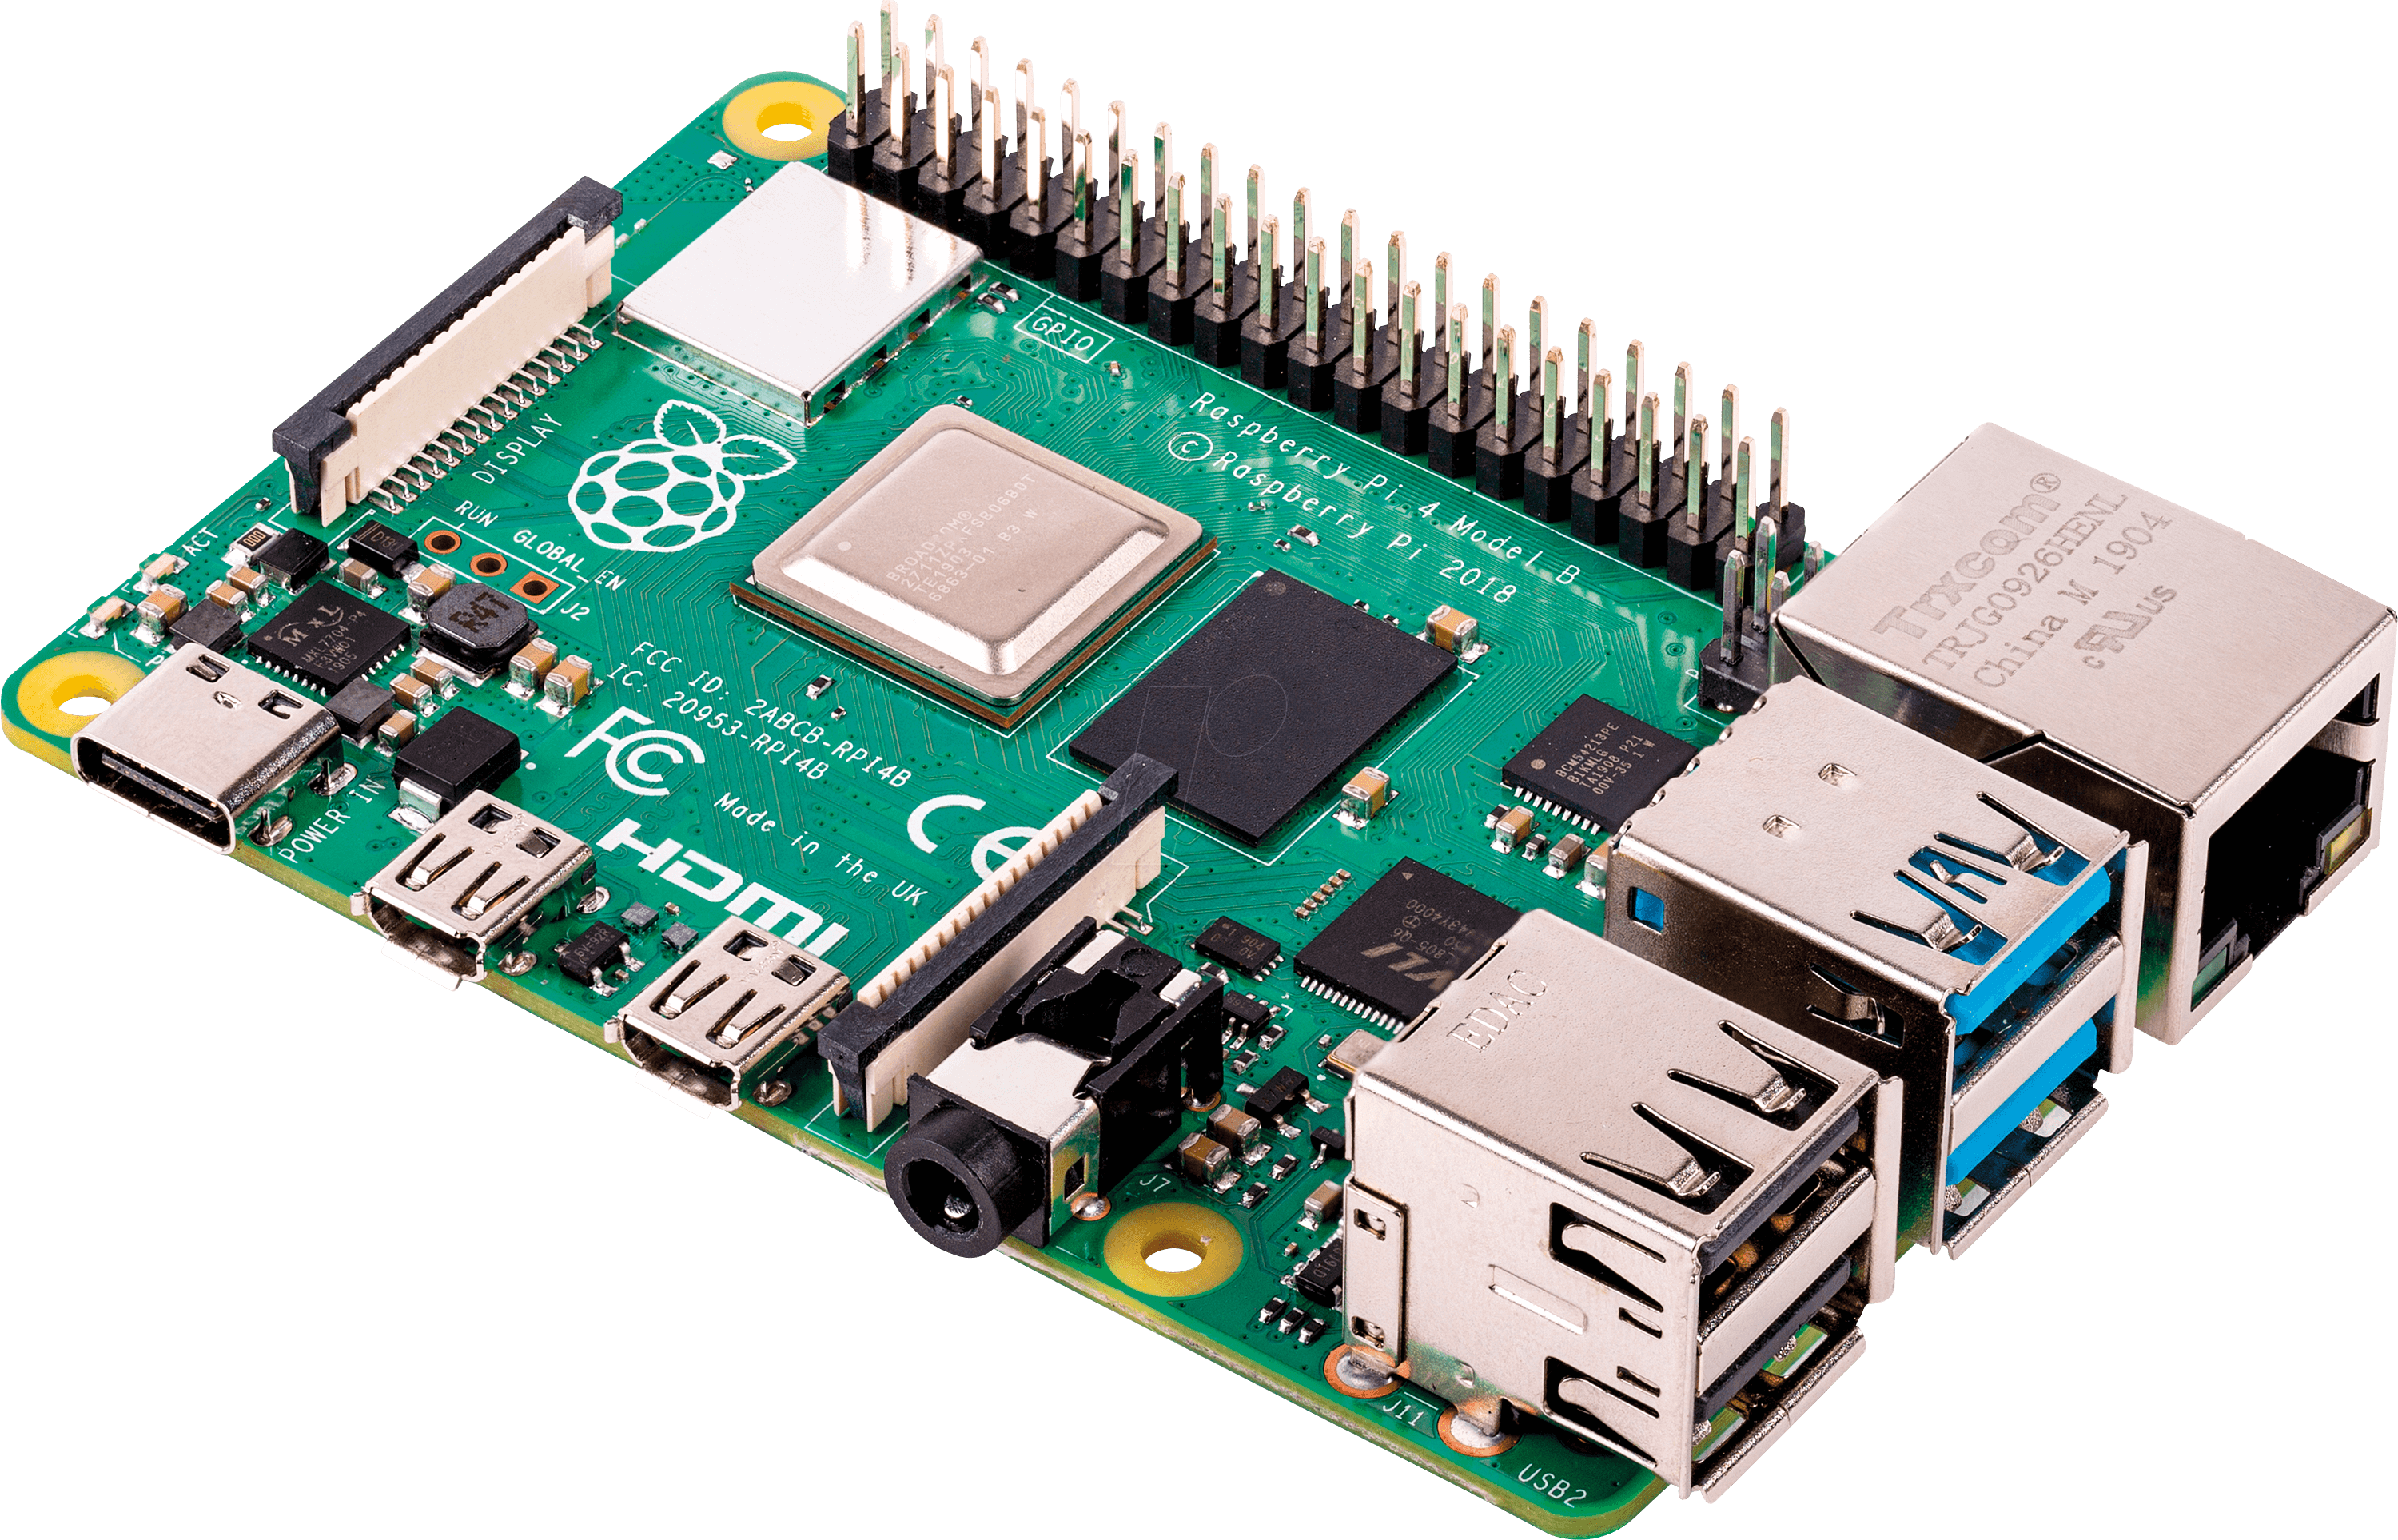
\includegraphics[width=0.8\textwidth]{./Bilder/raspberrypi_4.png}
    \captionof{figure}{Raspberry Pi 4}
    \label{img:raspberrypi}
\end{minipage}
\begin{minipage}{0.45\textwidth}
    \centering
    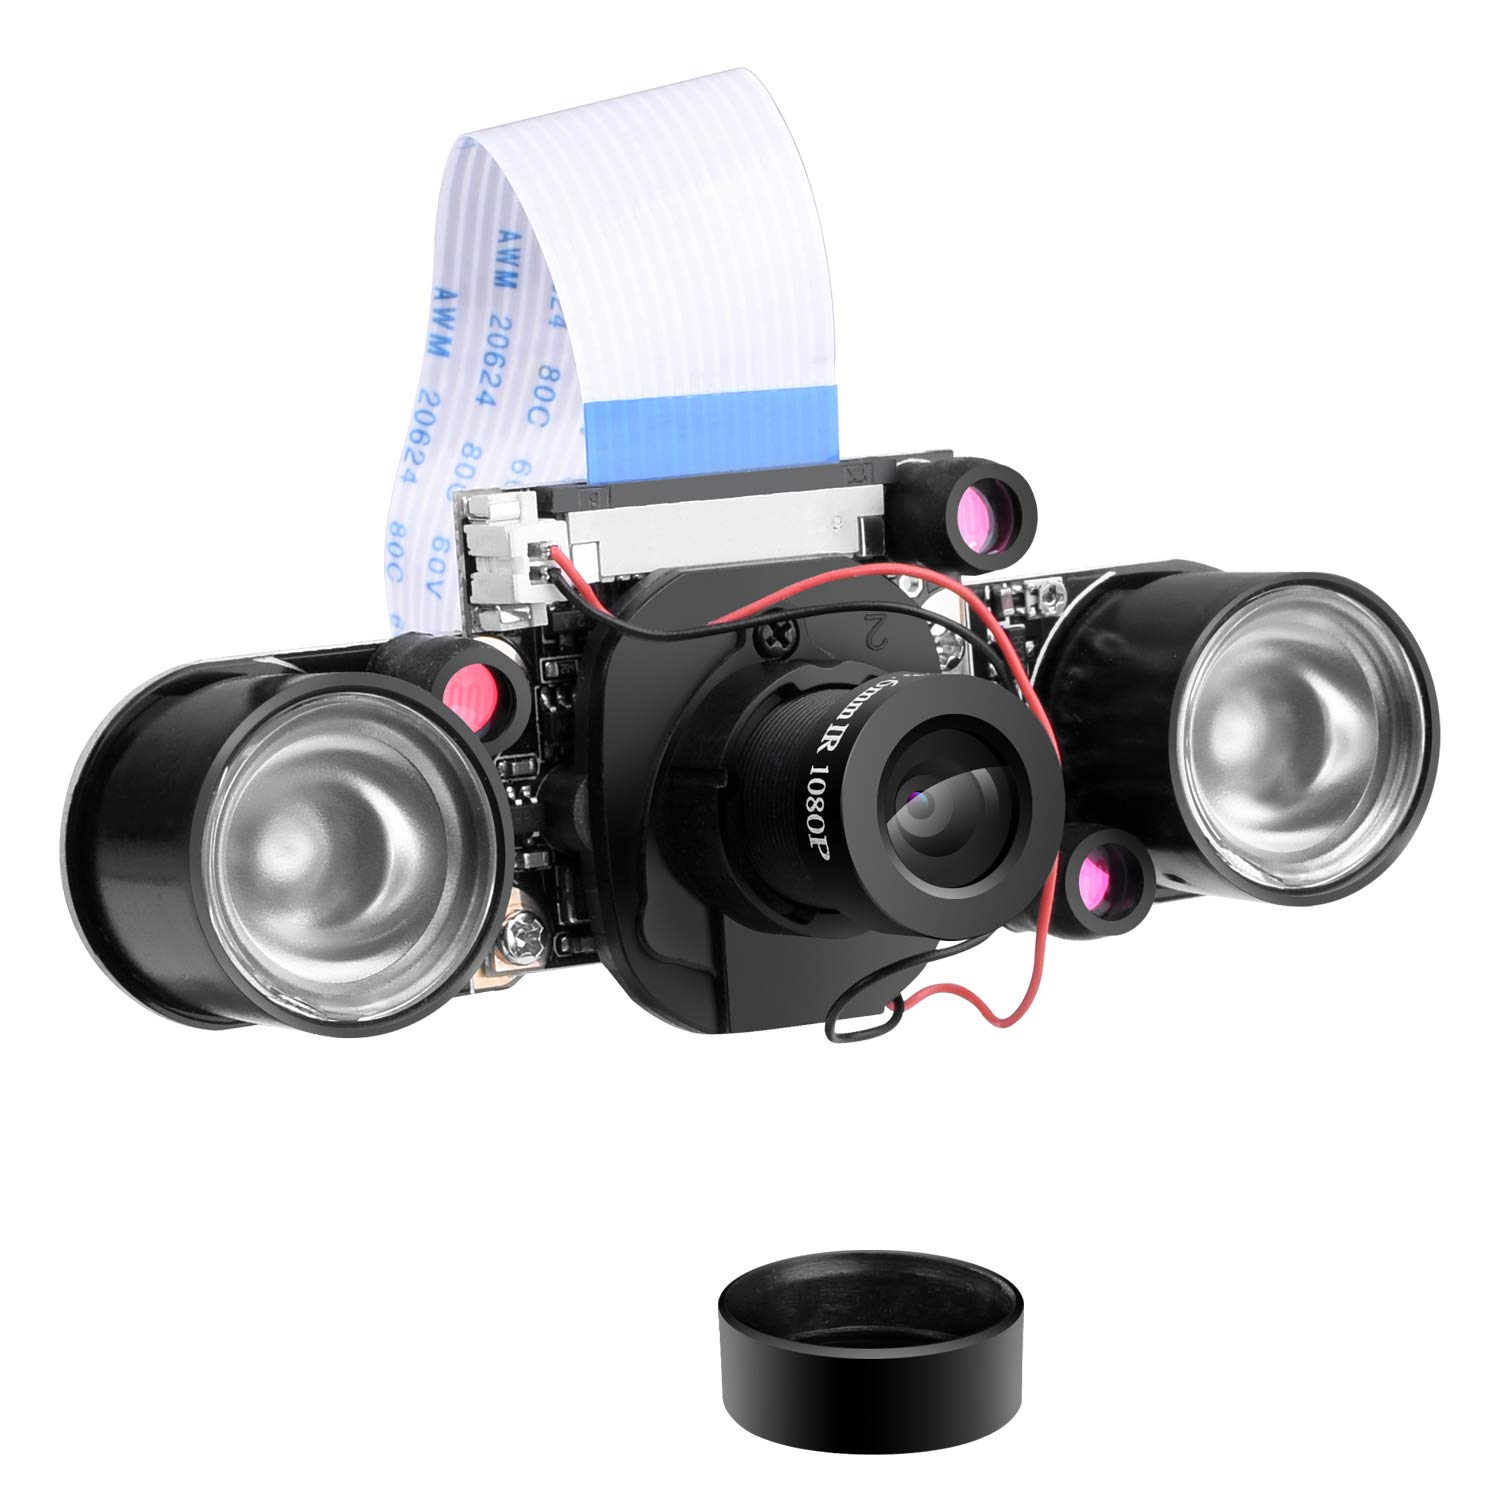
\includegraphics[width=0.8\textwidth]{longrunner.jpg}
    \captionof{figure}{Longruner Kamera Modul}
    \label{fig:rpicam}
\end{minipage}
\vspace{0.6cm}


Desweiteren wurde für eine mobile Internetverbindung 
der \textit{Huawei E3531 SurfStick} und zu Stromversorgnung
eine Powerbank verwendet.


% https://www.amazon.de/gp/product/B00HSZEY34/ref=ppx_yo_dt_b_asin_title_o00_s00?ie=UTF8&psc=1


\section{Implementierung/Software}

Die Implementierung der Anwendung wurde in Python vorgenommen und 
besteht aus den drei Scripten \texttt{main.py}, \texttt{detection.py}
und \texttt{connection.py}. Welche Folgend dargestellte Klassen 
implementieren.

\vspace{1cm}
\begin{tikzpicture} 

    
    
            \umlclass{Motion}{ 
              statickBackground : np.array
              }{ 
              + detectMotion() : bool \\
              + resetBackground() : void
            }
        
            \umlclass[y=-4]{InferenceModel}{ 
                string : plugin
                strin : device
                }{ 
                + createExecInferModel() : ExecInferModel
              }
        
            \umlclass[y=-2, x=6]{ExecInferModel}{ 
                shape : ioBlob\\
                detected : array
                }{ 
                + inferFrames() : status \\
                \# status[0] num infered\\
                \# status[1] num detected\\
                \# status[2] num saved\\
                - save() : void
                }
        
    
        \umlclass[x=11, y=-2]{Connection}{ 
            string logindata
            }{ 
            + login() : bool \\
            + connect() : server, port\\
            + send() : bool\\
            + disconnect() : bool\\
            + sendEmail(email, text) : boiol
          }

    
    \end{tikzpicture}
        
\vspace{1cm}

Dabei führt die Main Anwendung eine Dauerschleife aus, in der 
die Frames der Kamera erhalten werden. 

Die inferenz wird über das detection Script, welches die 
InferenceEngine implementier ausgeführt.
Das senden erkannter Ergebnisse erfolgt dann mithilfe 
des Detection Scripts.


Um trotz der langsamen Inferenz Zeit das Faster R-CNN 
verwenden zu können, galt es die Anwendung und die 
Zeitliche ausführungen der Inferenz so zu gestallten, 
das möglichst alle Frames, in welchen Tiere zu beobachten 
sein können, auch inferiert werden.

Dafür wurde die Annahme gemacht, dass zur Laufzeit der 
Anwendung häufig Zeiten sind in denen nichts zu inferieren 
ist, was durch eine Bewegungserkennung herausgefunden werden 
konnte.

Desweiteren wurde die Inferenz so implementiert, dass sie 
im gegensatz zur üblichen verwendung an keiner stelle Blockiert, 
wodurch durch zwischen Speichern von Bildern in denen 
Bewegung erkannt wurde trotz langsamerer Inferenzzeit alle 
Frames inferiert werden können.

Folgendes Diagramm zeigt schmematsch den groben Ablauf davon.

\vspace{1cm}


\begin{center}
\tikzset{
    desicion/.style={
        diamond,
        draw,
        text width=4em,
        text badly centered,
        inner sep=0pt
    },
    block/.style={
        rectangle,
        draw,
        text width=10em,
        text centered,
        rounded corners
    },
    arrow/.style={
        draw,
        >=latex,
        ->
    }
}


\begin{tikzpicture}
    \node (A) [desicion] {entschei\\dung};
    \node (B) [block, below of=A, node distance=3cm, text width=5em] {bock};
    \node (C) [block, right of=A, node distance=0.5\textwidth] {noch ein\\bock};


    \draw[arrow] (A) --  node [left, fill=white!30] {yes} (B);
    \draw[arrow] (A) -- node [below, near end] {crap} (C); 
    \draw[arrow] (B) -| node [near start, fill=white] {yes} (C);

\end{tikzpicture}

\end{center}

\subsection{Inferenz}

\subsubsection{Motion}

Die Bewegungserkennung wurde mithilfe der Library OpenCV implementiert, indem
zu beginn ein Frame als Refernz abgespeichert wurde.
Mit diesem konnten dann alle weiteren Input frames vergleichen werden 
indem der Abstand der einzelnen Pixel werte berechnet und gemittelt wird.
Beträgt dieser mehr als ein bestimmter threshhold wird das als Bewegung 
gewertet.

\subsubsection{Inferenz}

Die in Abschnitt \ref{sec:infertime} beschriebene asynchrone 
Inferenz wurde dahingehend abgeändert, dass nun theoretsch belibieg file 
Requests verwendete werden können und für den wait Befehl der 
Timeout auf 0ms gesetzt wurde und so der Ablauf nicht mehr Blockierend 
ist. Dadurch kann die Inferenz unabhängig von der Frequenz der 
von der Kamera erhaltenen Bilder ablaufen.
Auf eine richtige zuordnung der Inferenz ergebnisse zu dem 
jeweiligen verwendeten Frame war zu achten.


\begin{algorithm}[H]
    \caption{Asynchrone Inferenz, ohne Blockierung}
    \begin{algorithmic}
    \WHILE{\TRUE}
    \STATE capture FRAMES
        \FOR{ReqNr in all InferRequests}
            \STATE status \textbf{wait} for ReqNr
            \IF {status == 0}
                \STATE res = ReqNr.output
            \ENDIF
            
            \IF {Buffer != 0}
                \STATE preprocess ReqNr
                \STATE \textbf{statr} ReqNr
            \ENDIF

            \IF{res != NULL}
                \STATE process result
            \ENDIF
        \ENDFOR
    \ENDWHILE
    \end{algorithmic}
\end{algorithm}    



\subsection{Conncection/Verbindung}


Um eine Verbindung zwischen Raspberry Pi und Pc herzustellen, 
die unabhängig davon ob sich die geräte im selben 
Netzwerk befinden funktioniert, wurde eine Cloud Proxy Verbindung 
implementerit.

Dafür wurde der Dienst \textit{remot3.it} \cite{remoteit} verwendet, 
mit dem es möglich ist ohne Konfiguration des Routers eine
Netzwerkübergreifende Remote Verbindung zum Raspberry Pi herzustellen.

Da die Daten vom Raspberry aus automatisch gesendet werden sollen, 
wurde der Pc als Remote Gerät implementerit un auf dem Raspberry 
eine SSH Verbindung zum Pc hergestellt.


\begin{figure}[H]
    \centering
    \def\svgwidth{0.7\textwidth}
    \input{Bilder/diagram-connect.pdf_tex}
    \caption{}
    \label{}
\end{figure}


Dafür bot remot3.it eine API die es ermöglicht über Get und Post Requests
den Verbindung auf und Abbau zu automatisieren.

Gesendet wurden die Daten dann per SCP Command (Secure Copy Protocol), 
welches die aufgaebaute SSH Verbiindung verwendet.













% \input{Bilder/class_diagramm/class_diagramm.latex}

% \begin{minipage}{0.3\textwidth}
%     \centering
%     \input{Bilder/diagramme/class_detection.tex}    
% \end{minipage}
% \begin{minipage}{0.3\textwidth}
%     \centering
%     \input{Bilder/diagramme/class_connection.tex}
% \end{minipage}
% \begin{minipage}{0.3\textwidth}
%     \centering
%     \input{Bilder/diagramme/class_motion.tex}
% \end{minipage}

% oder

%\input{Bilder/diagramme/detection_package.tex}

% oder 





%Asynchrone inferenz
%https://docs.openvinotoolkit.org/latest/_demos_python_demos_object_detection_demo_ssd_async_README.html

% main
% \begin{algorithm}[H]
%     \caption{Main Program}
%     \begin{algorithmic}

%     %\STATE INIT EXEC_NET, CAM

%     \WHILE{\TRUE}
%         \STATE capture frame
        
%         \IF{frame has motion}
%             \STATE $buffer \leftarrow frmae$
%         \ENDIF

%         \IF{buffer is empty}
%             \STATE disconnect
%         \ENDIF

%         \STATE result = inferFrames (buffer)

%         \FOR{all results}
%             \STATE process results
%             \IF {saved}
%                 \STATE sendRequest = \TRUE
%             \ENDIF
        

%             \IF {no detectoin for 20 times}
%                 \STATE reset motion background
%                 \STATE delete buffer
%                 \IF {connected}
%                     \STATE disconnect
%                 \ENDIF
%             \ENDIF

%         \ENDFOR

%         \IF {send all every minute}
%             \STATE save current detections
%             \STATE sendRequest = \TRUE
%         \ENDIF

%         \IF{sendRequest == \TRUE}
%             \IF{not logged in}
%                 \STATE log in
%             \ENDIF

%             \IF{not connected}
%                 \STATE connect
%             \ENDIF

%             \STATE server, port $\leftarrow$ connection

%             \STATE sendRequest = \FALSE
%             \FOR{all saved images}
%                 \IF{send image $\rightarrow$ server, port}
%                     \STATE delete image
%                 \ELSE
%                     \STATE sendRequest = \TRUE
%                 \ENDIF
%             \ENDFOR

%         \ENDIF
%     \ENDWHILE


%     \end{algorithmic}
% \end{algorithm}



% \newpage

% \begin{center}
%     \rule{0.8\textwidth}{0.4pt}
%     \begin{lstlisting}[language=Python]
%         def infer_frames(Buffer, threshhold):
%             for idx, inferRequest in all inferRequests:
%                 status = inferRequest.wait(0) # nicht blockierend
%                 if status not ready:
%                     continue
                
%                 if idx in currentFrames:
%                     results = inferRequest.output
%                     frame = currentFrames[idx]

%                 if Buffer not empty:
%                     currentFrames[idx] = Buffer.pop()
%                     infer_frame = preprocess(currentFrames[idx])
%                     inferRequest.async_infer(infer_frame)

%                 if results or frame is None:
%                     continue

%                 for obj in all results:
%                     Class, Roi, Proba <- obj
%                     if Proba < threshhold:
%                         continue
                    
%                     coords <- Roi, frame.shape

%                     infered_frame = draw_rect(frame, coords)

%                     if proba > detectedObjects.proba
%                         replace detectedObjects

%                     if number of detections > x:
%                         send(frame)
                    
%     \end{lstlisting}
%     \rule{0.8\textwidth}{0.4pt}        
% \end{center}


% \centering\rule{0.6\textwidth}{0.4pt}
% \begin\centering{lstlisting}[language=Python]
%     def infer_frames():
%         for all requests:
%             do something \textbf{with} request

%             status = request.wait(0)
%             if status == done:
%                 res = requests.output
%                 frame = current[id]
% \end{lstlisting}
% \centering\rule{0.6\textwidth}{0.4pt}




% % inferenz
% \begin{algorithm}[H]
%     \caption{Asynchrone Inferenz}
%     \begin{algorithmic}
%     \WHILE{\TRUE}
%         \STATE capture Frame
%         \IF{Frame has Motion}
%             \STATE Buffer $\leftarrow$ Frame
%         \ENDIF
%         \FOR{$reqId$ = 0 to $reqMax$}
%             \IF {Model.reqests[$reqId$].wait(0)}
%                 \STATE result = Model.reqests[$reqId$].output
%                 \STATE inferedFrames $\leftarrow$ (result, currentFrames[$reqId$])
%                 \IF {Buffer not empty}
%                     \STATE currentFrames[$reqId$] $\leftarrow$ Buffer 
%                     \STATE inFrame = preprocess: currentFrames[$reqId$]
%                     \STATE Model.inferAsync($reqId$, inFrame)
%                 \ENDIF
%             \ENDIF
%         \ENDFOR
%         \RETURN inferedFrames
%     \ENDWHILE
%     \end{algorithmic}
% \end{algorithm}

% wobei die wait Funktion mit Timeout = 0 nicht blockierend ist.

% Dadurch war es möglich trotz langsamerer inferenz zeit als 
% capture zeit, durch zwischenspeichern alle frames zu inferieren, 
% unter der Annahme, das nur zeitweise bewegung erkannt und damit 
% inferiert werden muss.




\chapter{Zusammenfassung und Ausblick}\label{kap:zusammenfassungausblick}


Ziel der Arbeit war, es ein autonomes
Kamerasystem zur Wildtierkennung,
mithilfe Neuronaler Netze, zu entwickeln.
Dafür wurden vortrainierte, CNN basierte, 
Deep Learning Modelle zur Objekterkennung
auf einen geeigneten Datensatz trainiert.
Dadurch sollte es Möglich sein, nicht 
nur die Anwesenheit eines Tieres 
zu Erkennen, sondern auch eine 
Klassifizierung der Tierart 
vorzunehmen, wodurch das System
gezielter für eine bestimmte
Anwendung eingesetzt werden kann.
Zur Realisierung, wurde neben einem Raspberry
Pi, sowie einer nachtsichtgeeigneten 
Kamera, für die Inferenz der 
\textit{Neural Compute Stick 2}
von \textit{Intel} verwendet, um die 
Verarbeitung der Daten auf dem 
Gerät ausführen zu können.
\vspace{0.5cm}

Für das Training wurde ein Datensatz, 
bestehend aus 9 Wildtierklassen verwendet,
welcher aus \textit{OpenImages} herunter 
geladen werden konnte.
Anschließend wurden die Daten 
für das Training aufbereitet und
zur Evaluierung, in verschiedene 
Sets aufgeteilt.
Das Training wurde dann mithilfe des 
Frameworks \textit{Tensorflow} durchgeführt,
wobei die Modelle \textit{SSD} und
\textit{Faster R-CNN} mit verschiedenen
Basis CNN und Parameter-Einstellungen
verwendet wurden.
Durch anschließende Evaluierung, konnte 
festgestellt werden, welches modell sich,
bezogen auf Genauigkeit und Geschwindigkeit,
am besten für die Anwendung eignet.
Der letzte Schritt war es die Inferenz, zusammen 
mit dem Anwendungscode für den Raspberry Pi 
zu implementieren, wofür mit OpenVino gearbeitet 
wurde.
\vspace{0.5cm}

Die Evaluierung der Modelle zeigte, dass 
eine erhöhte Genauigkeit, mit einer 
langsameren Inferenzzeit einhergeht.
Verbessert werden konnte die Genauigkeit 
zum einen durch eine Augmentierung der Daten 
was eine größere Robustheit gegenüber anderer 
Datensätze mitsich brachte, und zum 
anderen durch verwenden des Faster 
R-CNN, mit welchem auch Tiere weiter 
weg erkannt werden konnten.
Die Performance der Inferenz konnte durch 
asynchrone Inferenzausführung und 
verwenden eines bewegungsmelders sowie 
zwischenspeichern der frames verbessert werden.
\vspace{0.5cm}


Auffällig war der hohe Energieverbrauch, 
der durch den Neural Compute Stick, die Kamera mit 
Infrarot LEDs sowie dem Internetstick für den 
Raspberry Pi zustande kam.


%
  
\end{document}